\documentclass[11pt, titlepage]{article}
\usepackage[onehalfspacing]{setspace} 
\usepackage{fullpage}
\usepackage{graphicx}
\usepackage{float} % needed for [H]
\usepackage{titlesec}
\usepackage{lineno}
\linenumbers
\newcommand{\wordcount}{\input{../results/wordcount.sum}}


\begin{document}
    \begin{titlepage}
    \begin{center}
            {\large IMPERIAL COLLEGE LONDON}
    \end{center}
    
    \vspace*{\fill}
    
    \begin{center}
        {\Huge How well do different mathematical models, e.g., based upon population growth (mechanistic) theory vs. phenomenological ones, fit to functional responses data across species?}
    
        \bigskip
        Kayleigh Greenwood

        \bigskip
        3/12/2021

        \bigskip
        Word Count:
        \wordcount

    \end{center}
    
    \vspace{\fill}
    
    \end{titlepage}

    \begin{abstract}
    write at the end
    1-2 lines on background
    1-2 lines on objectives
    1-2 lines on methods
    1-2 lines on main results
    1-2 lines on main conclusions + take home messages (dont be vague eg more work is needed or x is useful)
    about 200 words
    \end{abstract}

    \section*{Introduction}
    
    aim for 400 words, 3 paragraphs

    Microbial growth rates are important to understand in the context of food safety, as there are significant financial and health burdens of foodborne illnesses \cite{daniel2020burden}, \cite{world2015estimates}. It is important to be able to predict microbial growth as accurately as possible in order to reduce these impacts via precise estimates of shelf life and other characteristics of growth \cite{mcmeekin1996shelf}. The standard method for growth prediction used to be null hypothesis testing, however an increasingly popular alternative is mathematical modelling \cite{foegeding1997driving}. Growth models typically contain four phases; lag, exponential, stationary and death. The death phase is typically excluded in the context of food microbiology, as becuase food is almost certainly spoiled or unit by the time this phase begins, it is irrelevant \cite{ross2003modeling}, and therefore will not be considered throughout this paper. This approach consists of fitting various models to data, each representing a separate hypothesis, and using model selection to determine which model its the best. Model fitting is benefcial as it allows multiple hypothesis to be assessed and compared at once, as opposed to only being able to accept or reject a null hypothesis. Levins (1966) highlighted that the ideal model will never be feasbile, forming the basis of the complexity of modelling, and why there is no one uniform population model which spans population biology. Literature on microbial growth rates contains various models with countless combinations of assumptions and techniques. Commonly used models such as x and x prioritise realism and precision but sacrifce generality. On the other hand, popular general models which prioritise generality, such as x and y, make a trade off with precision.
    
    Both empirical and mechanistic models have been used throughout the literature for modelling microbial growth. Initially, empirical models were used which were derived from models outside of the microbial growth sector, such as the Gompertz and Logistic models. However, mechanistic models have since been developed, such as the Baryani model \cite{grijspeerdt1999estimating}. The benefits of recently developed mechanistic models are that the model's parameters have a theoretical basis, however, there will always be doubt around whether the underlying mechanisms that the results rely on are accurate \cite{lopez2004statistical}. This gives empirical models an advantage in that they don't have any risk associated with mechanistic assumptions, and although they have no theoretical basis, it is argued that explanation of a relationship/behaviour isn't necessary in order to predict it, and sometimes getting a prediction as precise as possible is the most important thing.
    
    The contrast described above is why neither empirical nor mechanistic models have prevailed over the other. In fitting both types of models to many samples within this dataset, I plan on using various model comparison/selection techniques to identify the strengths and weaknesses of the two modelling approaches in the context of microbial growth rates. By identifying the unique statistical aspects of each model I have aimed to discover if empirical or mechanistic models are best suited to microbial growth hypotheses.

    \section*{Methods}

    \subsection*{Data}
    I used an existing database to model microbial growth rate data in this study. The logistic growth data allowed me to draw conclusions about the studied models' compatibility with microbial growth rates by modelling bacterial abundance as the response variable, against time as the explanatory variable. This explanatory/response dynamic in microbial biology allows conclusions and theories to focus on the extent to which time affects microbial growth, and how big of an effect this is. The data contains measures of bacterial abundance over time, across various combinations of other variables. The dataset comprises 4387 observations across 10 variables, however any entries with negative time or abundance values were excluded, leaving 4294 observations for further analysis. Sample groups were sub-divided according to species, temperature, medium and experiment, resulting in 277 subsets. 


    \subsection*{Models}
    To test the suitability of empirical, linear models for microbial growth rate studies, I used a cubic polynomial. The exponential nature of growth means that the log is normally plotted in order to normalize variance, causing the data to behave in a sigmoidal fashion \cite{zwietering1990modeling}. A cubic polynomial has two peaks, and therefore three separate areas, which is the same amount of distinct areas as a growth curve has when studied in microbial growth, suggesting fitting this model would work well as the shape of a cubic curve resembles the shape of a sigmoidal behaviour of the growth rates. For the representative mechanistic model, i chose to fit the Logistic model. The Logistic model is a non-linear model, which I chose to plot because of it's competitive advantage in the estimation of when the death phase has been reached(the maximum value/carrying capacity). Although the death phase itself is not explicitly relevant to microbial growth, a parameter estimate of carrying capacity as accurate as what this model produces has importance in further analysis abilities. Being able to predict carrying capacity as well as the Logistic Model does means that estimates of other values and parameters beyond this analysis are improved. 

    \subsection*{Model fitting}
    I fitted the linear model with ordinary least squares 
    Describe the mathematical models i fitted and compared to the data, and which methods i used to do this.

    \subsection*{Model selection}
    Describe how i compared and selected models and why i used the methods i did (AIC/BIC)

    \subsection*{Computing tools}
	Due to R being initially formatted as a statistical language, i used R scripts for the majority of my computing, with specialist shell and python scripts for specific tasks. R's syntax made using it for data preparation, model fitting, plotting and analysis more seamless than trying to do similar tasks in Python, and R has especially superior abilities in terms of data visualisation. Despite this, Python's subprocess module made it the perfect vessel through which to run the workflow. Finally, I used bash as a script to aid in the compilation of the LaTeX code by using texcount. 
    

    \section*{Results}

    can subsection by hypotheses
    give averages of variables (exp and resp) eg mean and SD
    if p is really small say p < x, dont report power
    What  were  the  results of  your hypothesis  tests,  in  the  order  you describe  them  in  the Methods?
    describe hypothesis in same order as in results and intro

    \begin{figure}[H]
    \centering
    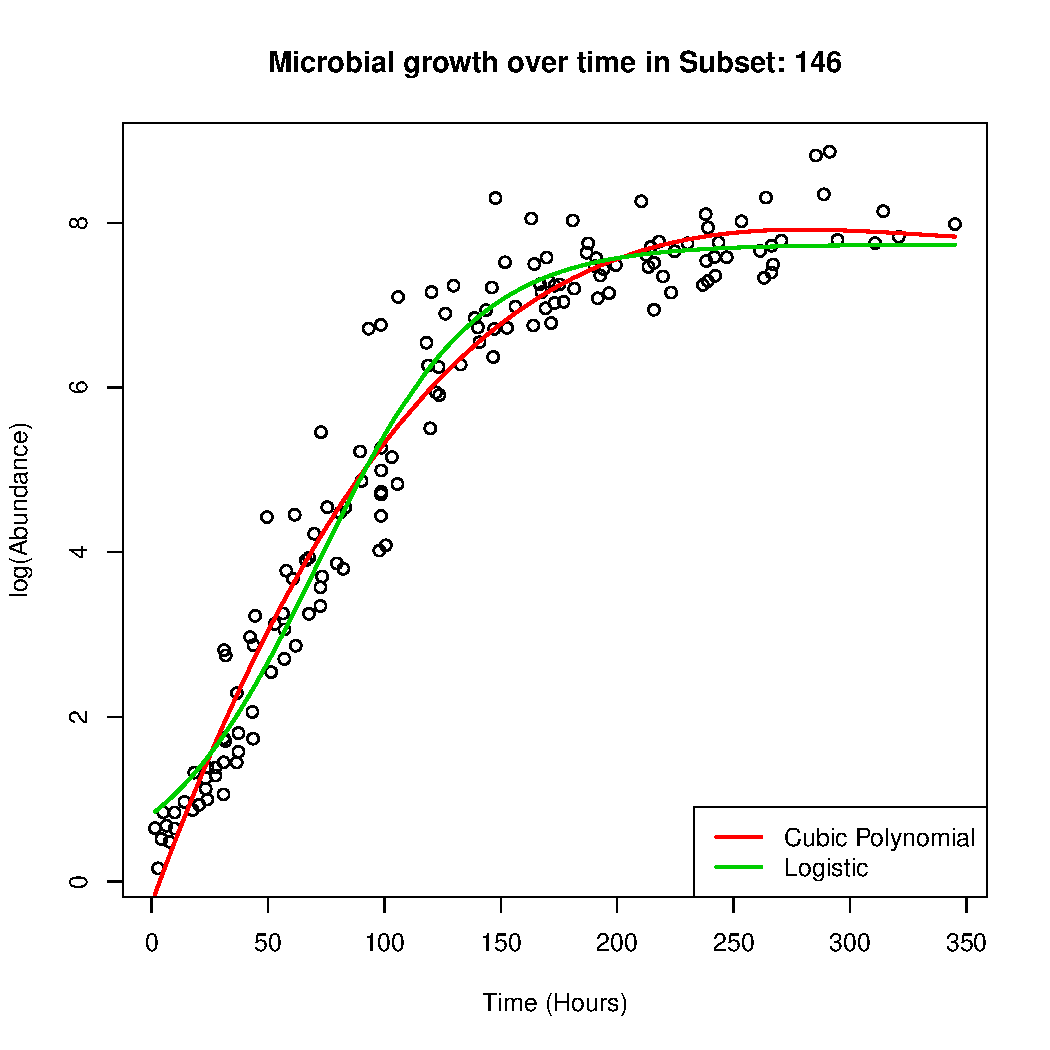
\includegraphics[scale=0.75]{../Plots/PlotID146.pdf}
    %TC:ignore
    \caption{this is a plot of a cubic polynomial and the logistic model fitted to one of the subsets within the dataset.}
    %TC:endignore
    \end{figure}

    \begin{figure}[H]
    \centering
    \includegraphics[scale=0.5]{../results/AIC.pdf}
    %TC:ignore
    \caption{AIC values of subsets}
    %TC:endignore
    \end{figure}

        \begin{figure}[H]
    \centering
    \includegraphics[scale=0.5]{../results/RSS.pdf}
    %TC:ignore
    \caption{RSS values for subsets}
    %TC:endignore
    \end{figure}

    \section*{Discussion}

    reminder of aims
    tie together results / key findings
    give results broader context - implications
    add more referencing
    what do we know now that we didnt before
    what is the chain of logic and results that means we know it (remember not to repeat anything from results section)
    extent to which original aims have been satisfied
    discuss limitations of my study and future work to address limitations
    what would i do differently if i had more time
    conclude emphasising how this study in this system is of interest to people who work on other things, or other systems

    \bibliographystyle{apalike}

    \bibliography{ReportBiblio}
\end{document}